% Options for packages loaded elsewhere
\PassOptionsToPackage{unicode}{hyperref}
\PassOptionsToPackage{hyphens}{url}
%
\documentclass[
]{article}
\usepackage{amsmath,amssymb}
\usepackage{iftex}
\ifPDFTeX
  \usepackage[T1]{fontenc}
  \usepackage[utf8]{inputenc}
  \usepackage{textcomp} % provide euro and other symbols
\else % if luatex or xetex
  \usepackage{unicode-math} % this also loads fontspec
  \defaultfontfeatures{Scale=MatchLowercase}
  \defaultfontfeatures[\rmfamily]{Ligatures=TeX,Scale=1}
\fi
\usepackage{lmodern}
\ifPDFTeX\else
  % xetex/luatex font selection
\fi
% Use upquote if available, for straight quotes in verbatim environments
\IfFileExists{upquote.sty}{\usepackage{upquote}}{}
\IfFileExists{microtype.sty}{% use microtype if available
  \usepackage[]{microtype}
  \UseMicrotypeSet[protrusion]{basicmath} % disable protrusion for tt fonts
}{}
\makeatletter
\@ifundefined{KOMAClassName}{% if non-KOMA class
  \IfFileExists{parskip.sty}{%
    \usepackage{parskip}
  }{% else
    \setlength{\parindent}{0pt}
    \setlength{\parskip}{6pt plus 2pt minus 1pt}}
}{% if KOMA class
  \KOMAoptions{parskip=half}}
\makeatother
\usepackage{xcolor}
\usepackage{graphicx}
\makeatletter
\def\maxwidth{\ifdim\Gin@nat@width>\linewidth\linewidth\else\Gin@nat@width\fi}
\def\maxheight{\ifdim\Gin@nat@height>\textheight\textheight\else\Gin@nat@height\fi}
\makeatother
% Scale images if necessary, so that they will not overflow the page
% margins by default, and it is still possible to overwrite the defaults
% using explicit options in \includegraphics[width, height, ...]{}
\setkeys{Gin}{width=\maxwidth,height=\maxheight,keepaspectratio}
% Set default figure placement to htbp
\makeatletter
\def\fps@figure{htbp}
\makeatother
\setlength{\emergencystretch}{3em} % prevent overfull lines
\providecommand{\tightlist}{%
  \setlength{\itemsep}{0pt}\setlength{\parskip}{0pt}}
\setcounter{secnumdepth}{-\maxdimen} % remove section numbering
\ifLuaTeX
  \usepackage{selnolig}  % disable illegal ligatures
\fi
\IfFileExists{bookmark.sty}{\usepackage{bookmark}}{\usepackage{hyperref}}
\IfFileExists{xurl.sty}{\usepackage{xurl}}{} % add URL line breaks if available
\urlstyle{same}
\hypersetup{
  hidelinks,
  pdfcreator={LaTeX via pandoc}}

\author{}
\date{}

\begin{document}

\hypertarget{linear-regressionlec1}{%
\subsection{Linear Regression(lec1)}\label{linear-regressionlec1}}

\hypertarget{notation-and-expression}{%
\subsubsection{notation and expression}\label{notation-and-expression}}

我们使用以下 notation:

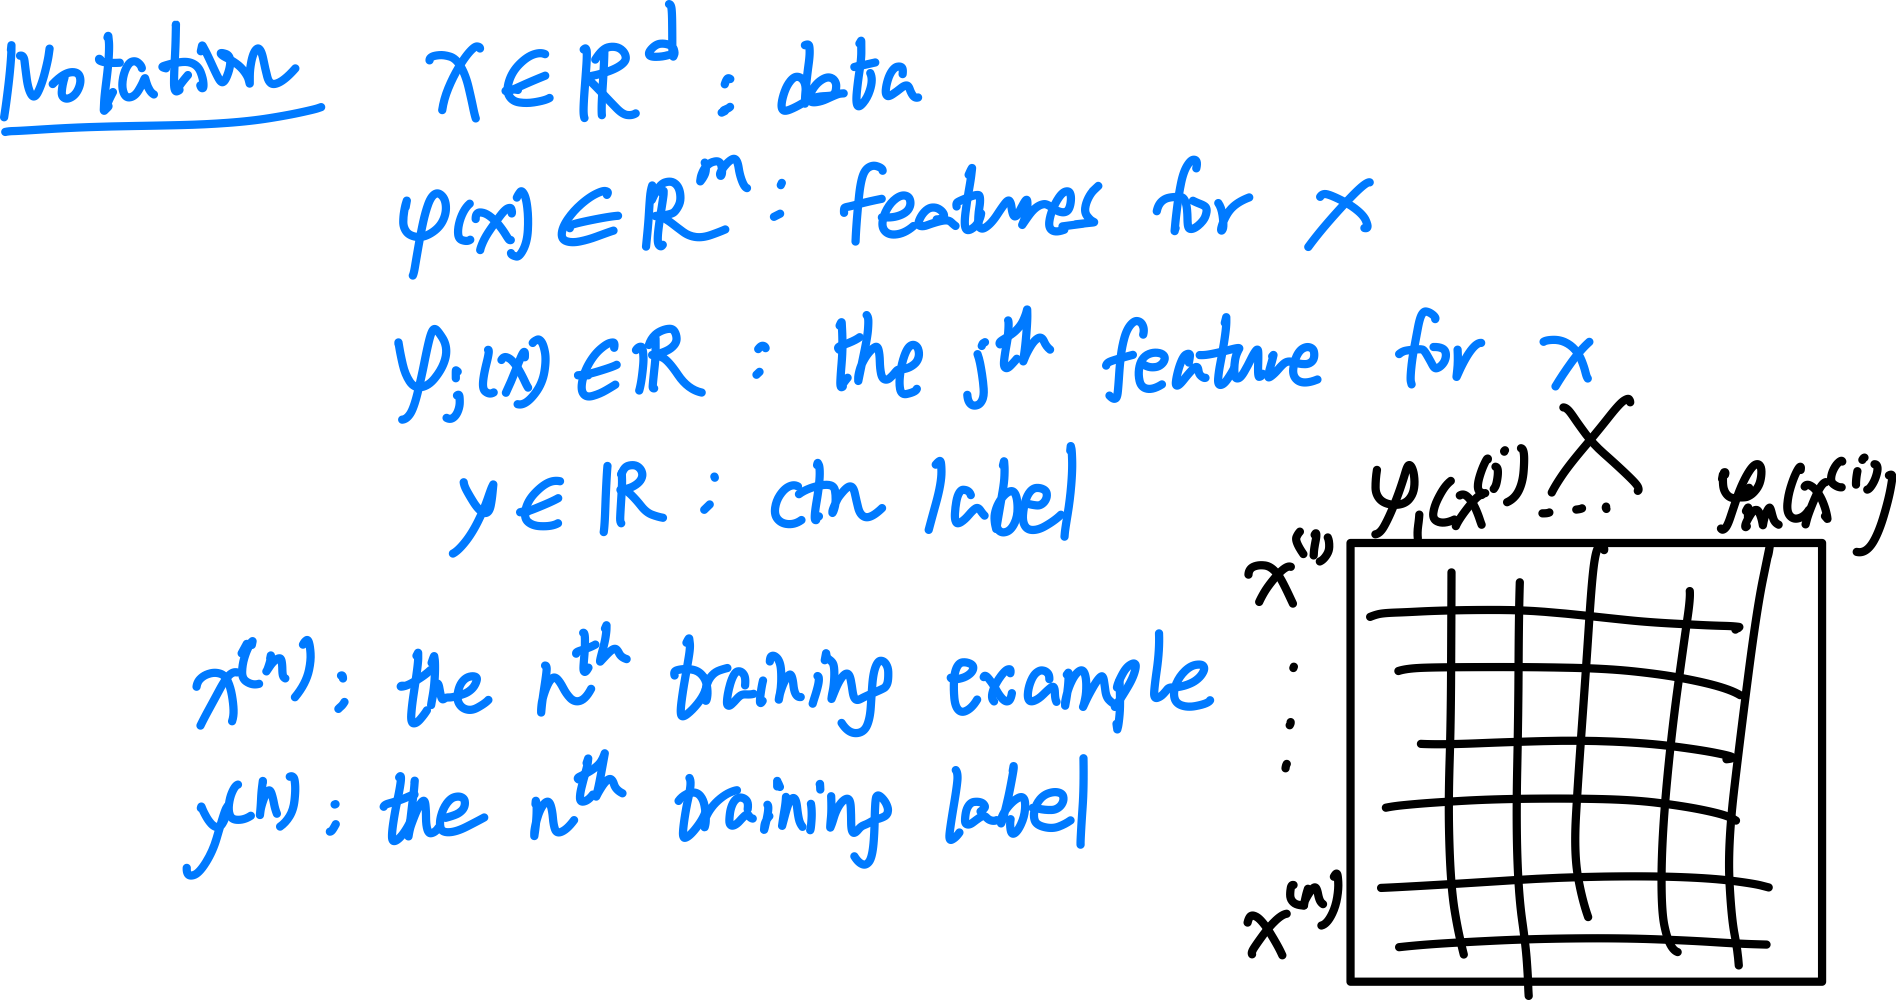
\includegraphics{/Users/fanqiulin/Desktop/cse-545_ML-notes/lec-notes/Linear_Regression.assets/lec1-notation.png}

\textbf{(generalized) linear regression 的定义:}\\
给定 \(N\) 个 data points \(\{(x^{(n)},y^{(n)}) \}_{n=1,\cdots, N}\)
where each \(x^{(n)}\in\mathbb{R}^d,y^{(n)}  \in\mathbb{R}\),
以及预先设定好的 \(M\) 个 basis functions
\(\{ \phi_i(x)\}_{i=1,\cdots, M}\) 用以表示 \(M\) 个 features;

我们通过建立一个
\(h(x,w): \mathbb{R}^d \times \mathbb{R}^M \rightarrow  \mathbb{R} = \sum_{i=0}^{M-1} w_i \phi_i(x)\),
使其关于 \(w\) 线性, 以找到一组参数 \(w \in \mathbb{R}^M\), 使得
\(h(x^{(n)},w)\) 能够近似 \(y^{(n)}\) for each \(n\), with respect to
the loss function we define to measure the distance between two vectors.

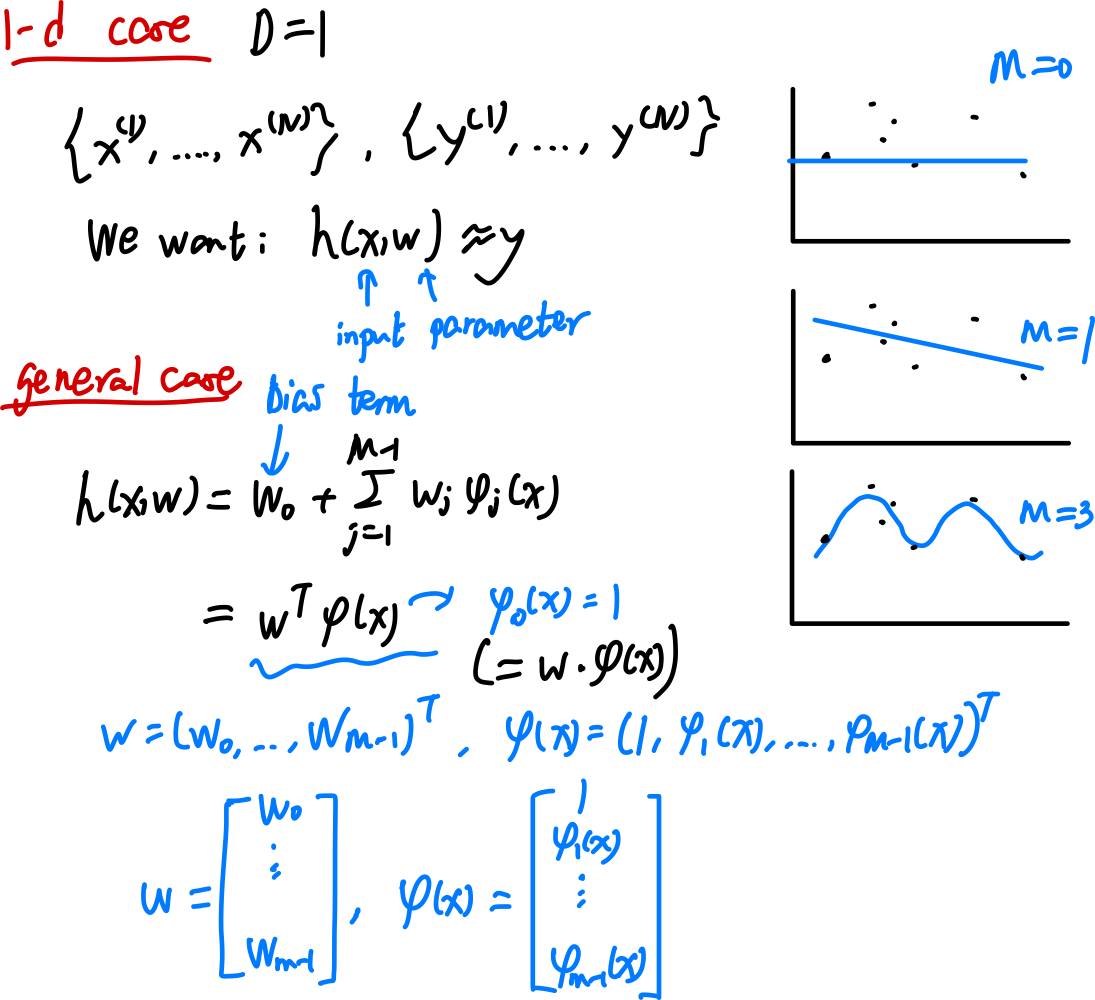
\includegraphics{/Users/fanqiulin/Desktop/cse-545_ML-notes/lec-notes/Linear_Regression.assets/lec1(expression).png}

Remark: 注意 linear regression 指的是 \(y\) 和参数 \(w\) 之间是 linear
的, 而不是说 \(y\) 和 input \(x\) 之间是 linear 的. 我们可以选择
nonlinear 的 basis funtions 来 encode \(x\) 来表示 features 的特性,
比如我们可以选择:

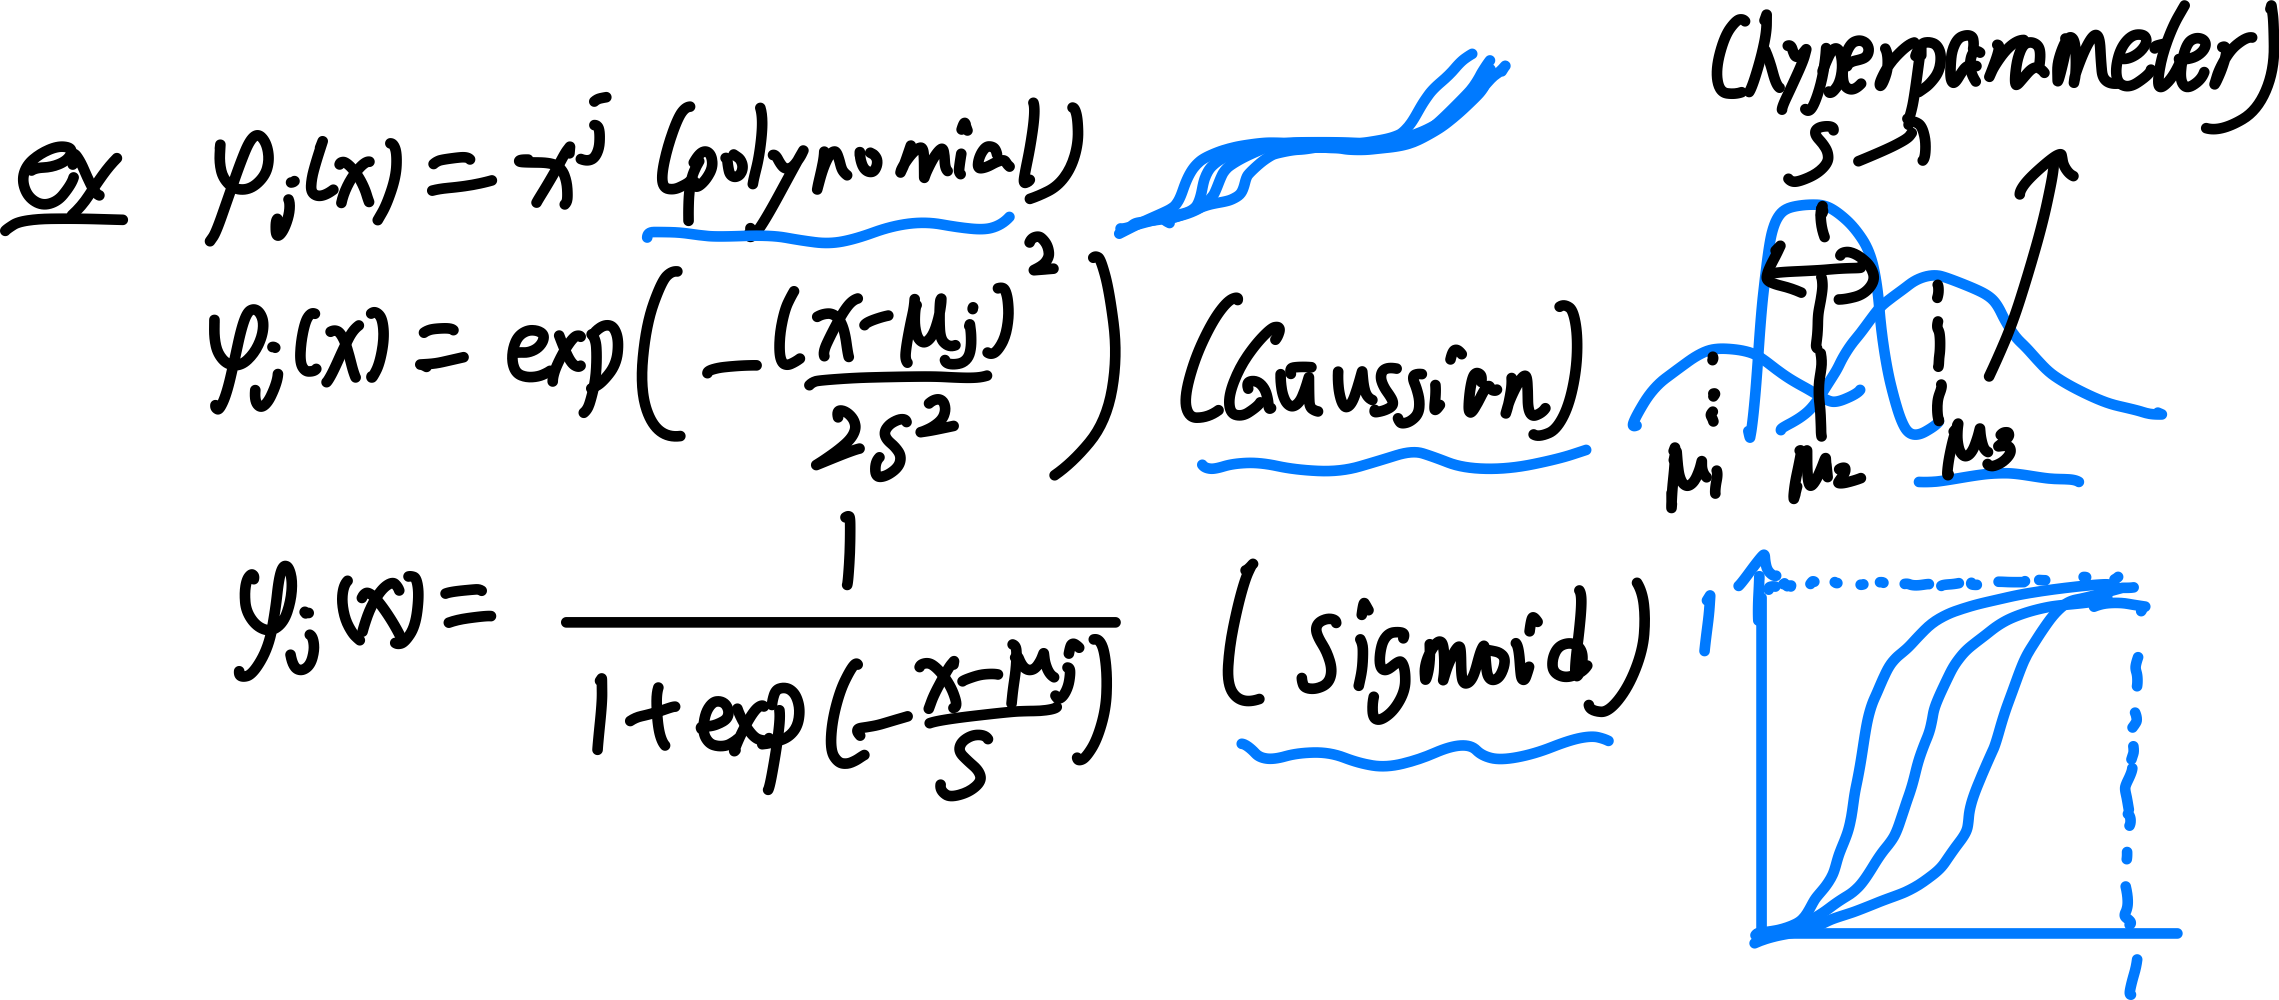
\includegraphics{/Users/fanqiulin/Desktop/cse-545_ML-notes/lec-notes/Linear_Regression.assets/lec1-basis.png}

\hypertarget{loss-function-sum-of-squared-error}{%
\subsubsection{loss function: sum of squared
error}\label{loss-function-sum-of-squared-error}}

这个 loss function 衡量两个 vectors 之间的距离, 目的是衡量
\(y \in \mathbb{R}^N\) 和 \(h(x,w) \in \mathbb{R}^N\) 这两个 vectors
的差距. 实际上就是它们 difference 的 \(L_2\)-norm 的平方.

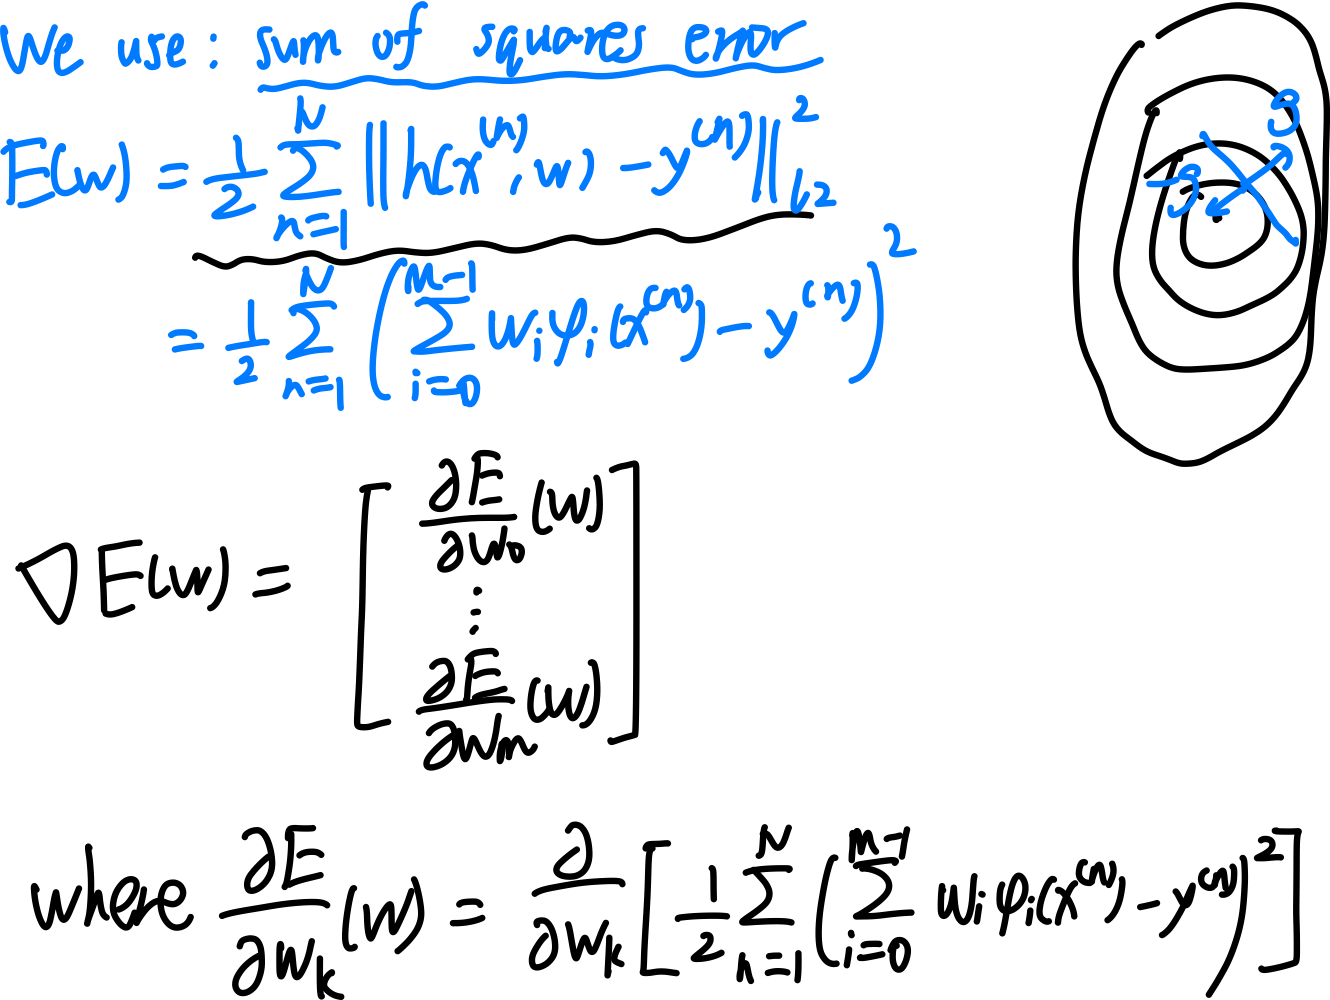
\includegraphics{/Users/fanqiulin/Desktop/cse-545_ML-notes/lec-notes/Linear_Regression.assets/lec1-loss.png}

\hypertarget{gradient-of-sum-of-squared-error}{%
\subsubsection{gradient of sum of squared
error}\label{gradient-of-sum-of-squared-error}}

我们下面首先通过求 \(\nabla E(w)\) 的每个 entry
\(\frac{\partial E}{\partial w_k}(w)\) 来写出这个 gradient.

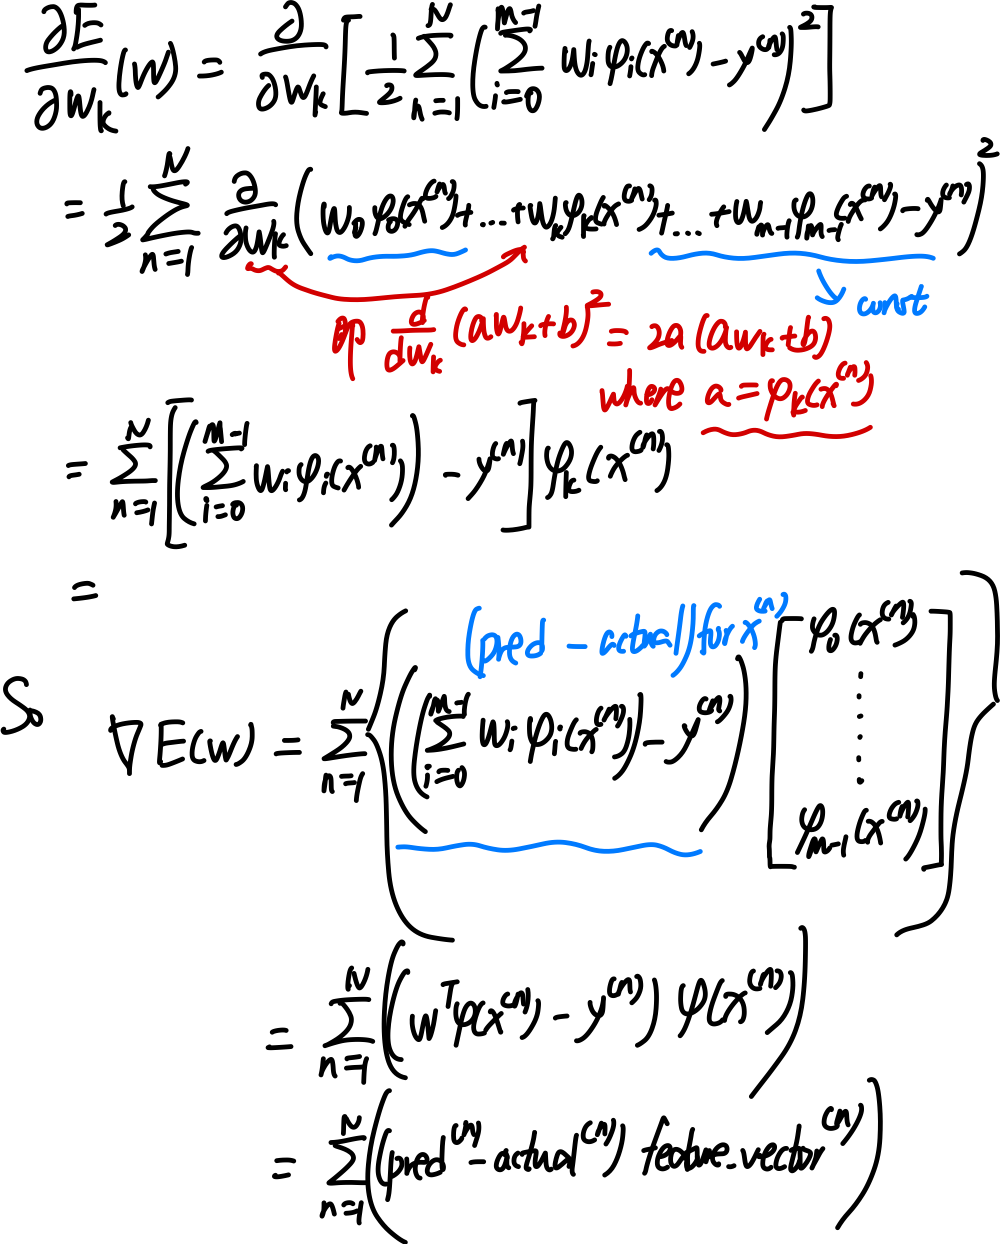
\includegraphics{/Users/fanqiulin/Desktop/cse-545_ML-notes/lec-notes/Linear_Regression.assets/lec1-gradient.png}

\hypertarget{batch-vs-stochastic-gd}{%
\subsubsection{batch v.s. stochastic GD}\label{batch-vs-stochastic-gd}}

我们通过迭代降低 gradient 来降低 loss function 的值, 从而优化 weight
vector.

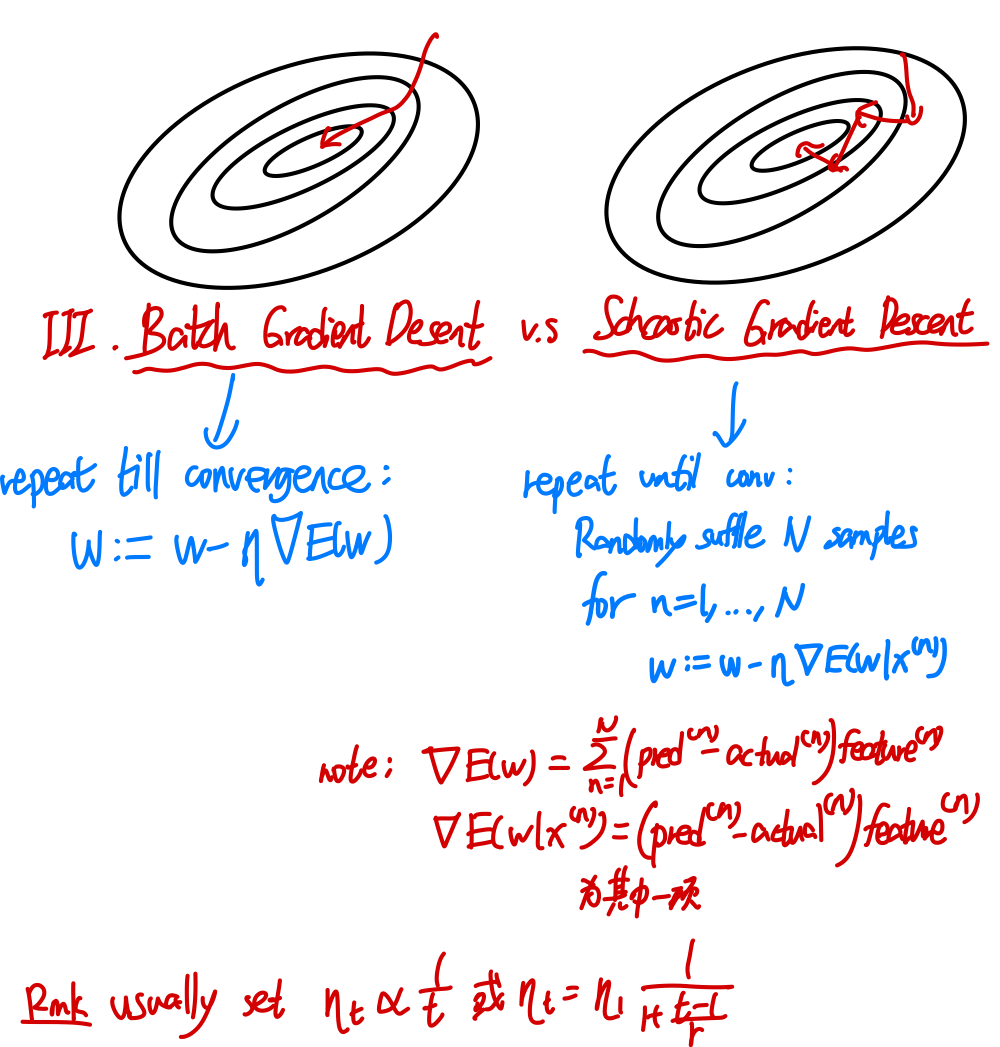
\includegraphics{/Users/fanqiulin/Desktop/cse-545_ML-notes/lec-notes/Linear_Regression.assets/lec1-descent.png}

(More practically, 我们可以采用 minibatch SGD: 即在 batch GD 和 SGD
之间, 每次选择一小部分 samples, 称为一个
\textbackslash textbf\{minibatch\}, 在这个 minibatch 上进行 GD.)

\hypertarget{linear-regressionlec2}{%
\subsection{Linear Regression(lec2)}\label{linear-regressionlec2}}

\hypertarget{vectorization}{%
\subsubsection{vectorization}\label{vectorization}}

我们可以把每个 \(x^{(n)}\) 的 features 写成一个 row vector, 并 stack up
\(N\) 个 row vectors, 成为一个 \(N\times M\) 的 matrix \(\Phi\). 从而:

\[h(x,w) = \Phi w\]

vectorization 的好处是: 1. 便于手算; 2. computer 可以进行并行计算.\\
\textbackslash pic{[}0.6{]}\{assets/lec2-vect.png\}\\
计算得 linear regression 的 loss function 为:

\[E(w) = \frac{1}{2}w^T \Phi^T \Phi w - w^T \Phi^T y + \frac{1}{2}y^T y\]

\hypertarget{vector-form-gradient-ux4ee5ux53ca-closed-form-sol}{%
\paragraph{vector form gradient 以及 closed-form
sol}\label{vector-form-gradient-ux4ee5ux53ca-closed-form-sol}}

如果

\[\nabla E(w) = y\]

有一个 closed form solution, 那么这个 solution 一定是一个 local min/max,
从而 possibly 成为一个 global min. (并且 we know, \textbf{如果 \(E\)
是个 convex 的函数, 那么一定是 global min!})

为了计算 closed form solution, 我们首先要给出 \(\nabla E(w)\) 的 matrix
form 表达式. \textbackslash{}\\
这里首先引入 linear form 和 quadratic form 的 gradient:

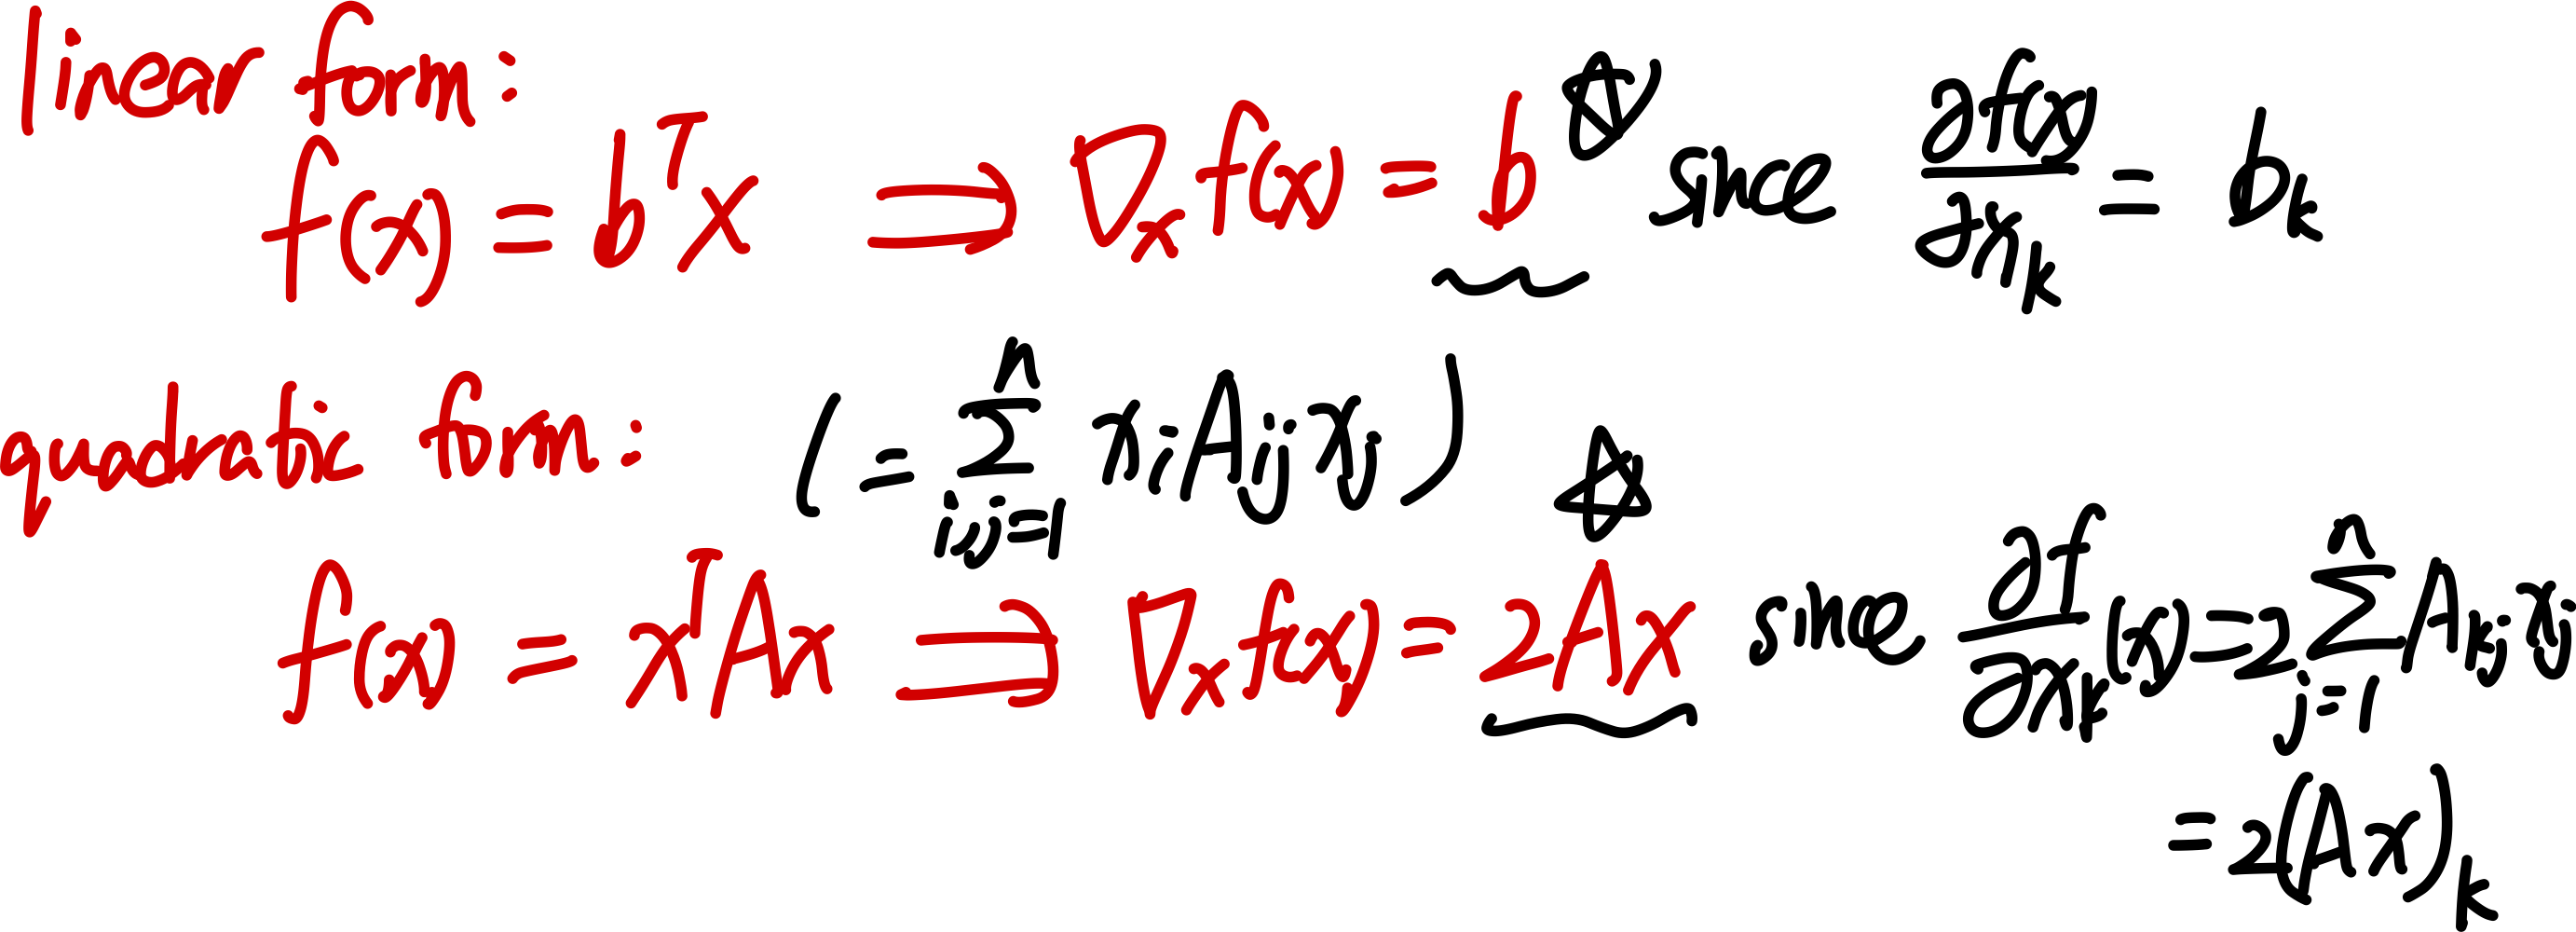
\includegraphics{/Users/fanqiulin/Desktop/cse-545_ML-notes/lec-notes/Linear_Regression.assets/lec2-diff.png}

我们发现: \(E(w)\) 就是一个 \(w\) 的 quadratic form, 一个 \(w\) 的
linear form 和一个 const 的组合. 从而可以求出:

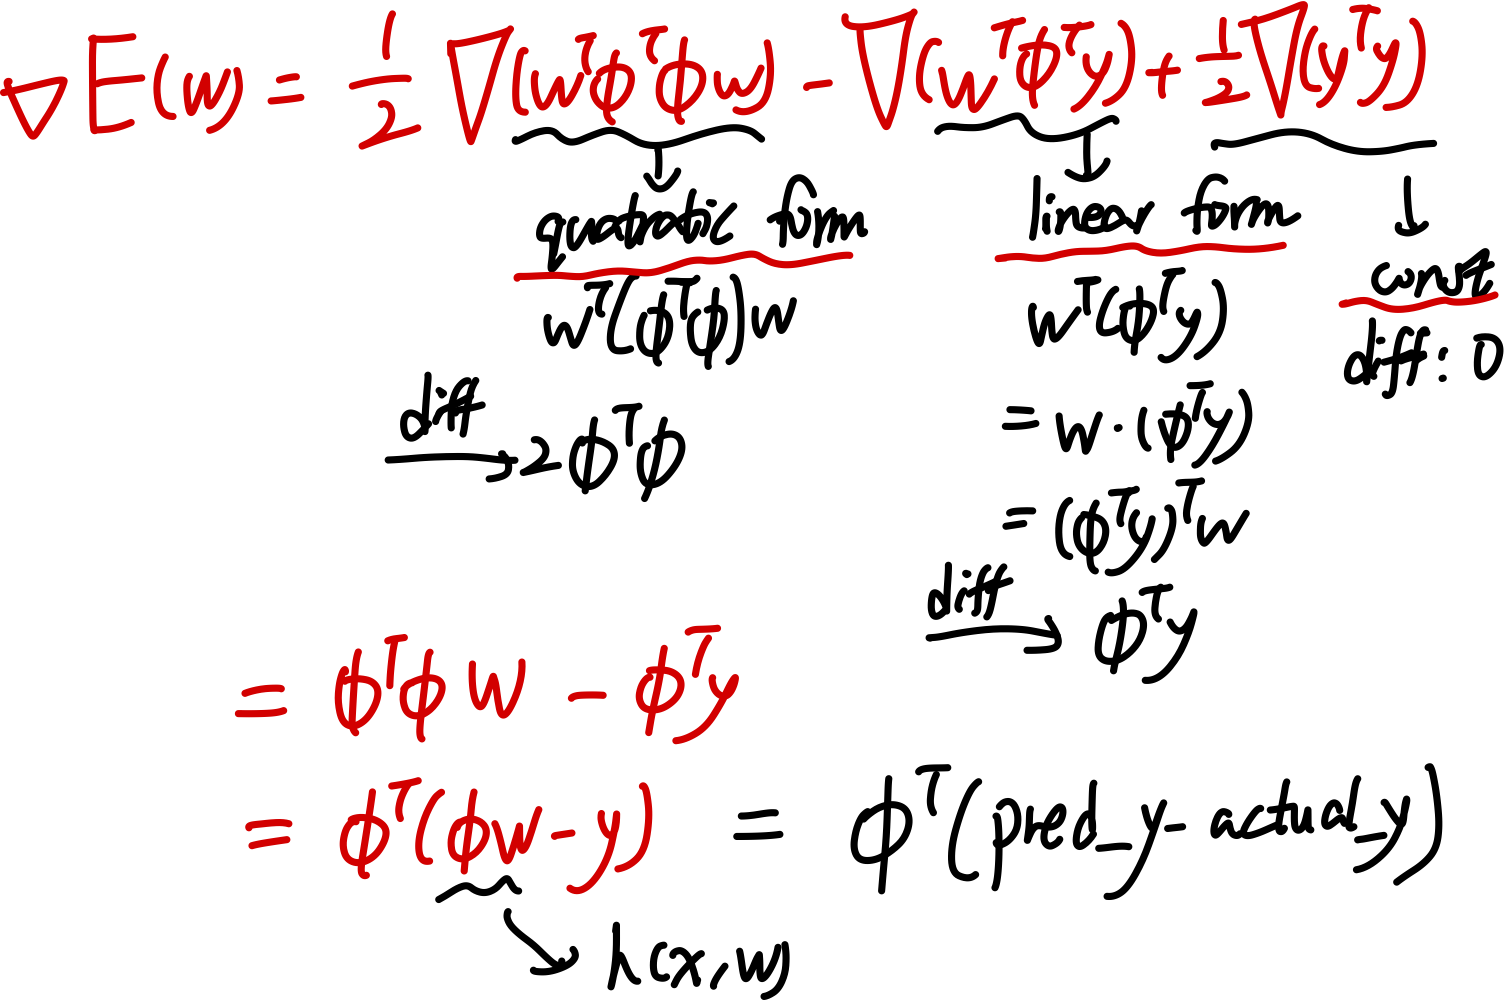
\includegraphics{/Users/fanqiulin/Desktop/cse-545_ML-notes/lec-notes/Linear_Regression.assets/lec2-grad.png}

从而我们得到 closed form solution (if exists):

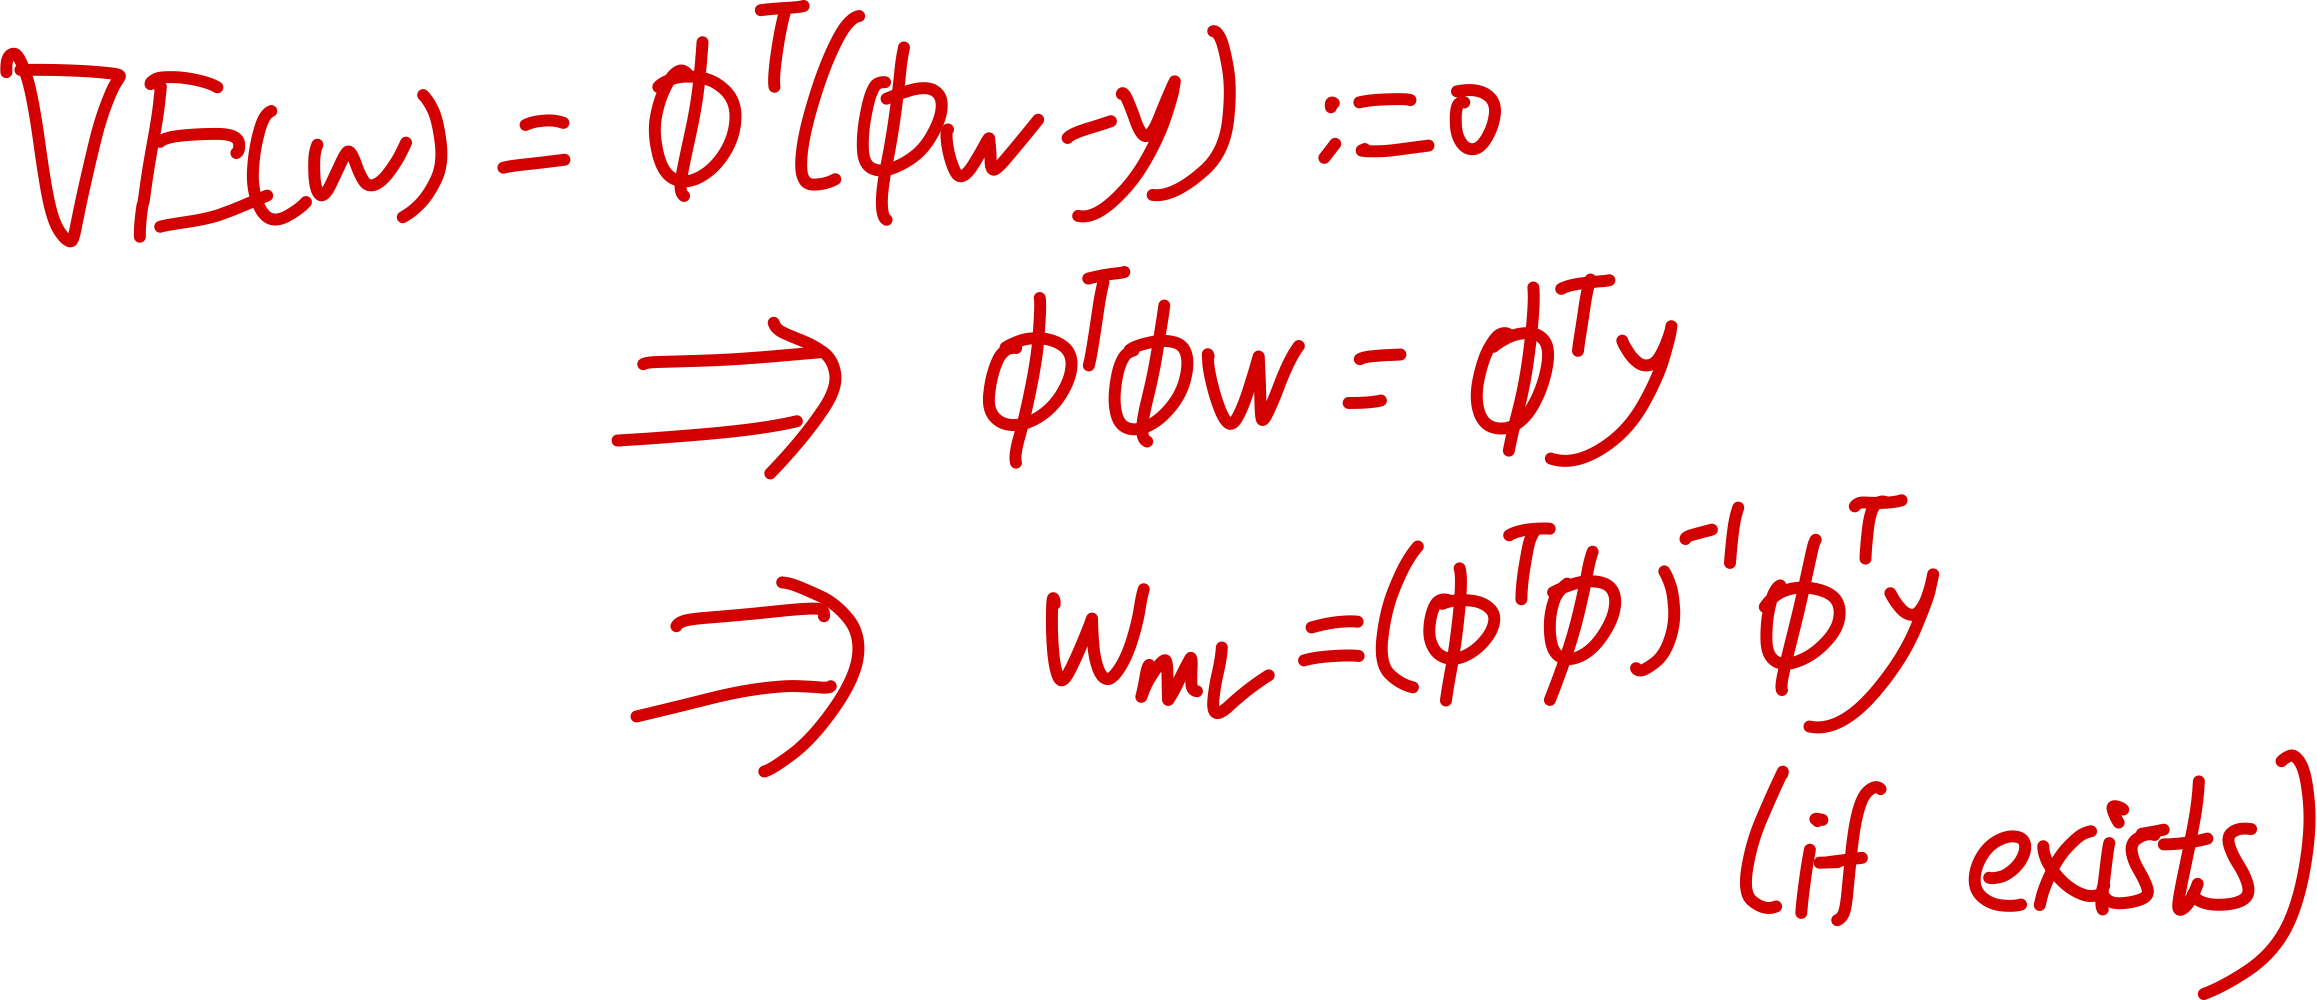
\includegraphics{/Users/fanqiulin/Desktop/cse-545_ML-notes/lec-notes/Linear_Regression.assets/lec2-closed.png}

因而 closed form exists iff \(\Phi^T\Phi\) 可逆, iff \(\Phi\) 可逆.\\
并且 recalll in linear algebra:
\textbf{\(rank(\Phi^T\Phi) = rank(\Phi)\).}\\
因而, \textbf{closed form exists iff \(M >= N \) 且 \(rank(\Phi) = N\)}

\hypertarget{overfitting}{%
\subsubsection{overfitting}\label{overfitting}}

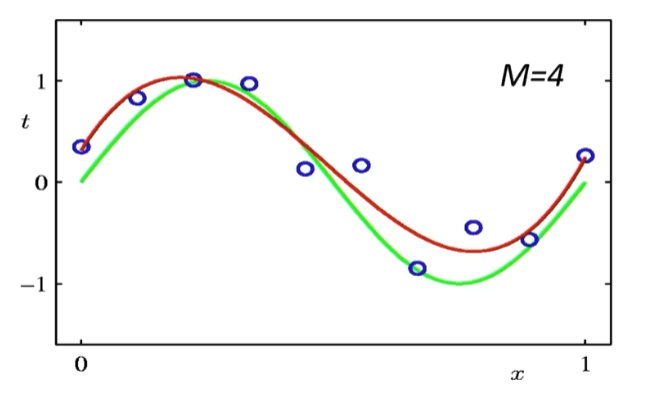
\includegraphics{/Users/fanqiulin/Desktop/cse-545_ML-notes/lec-notes/Linear_Regression.assets/Screenshot 2025-01-21 at 18.11.31.png}

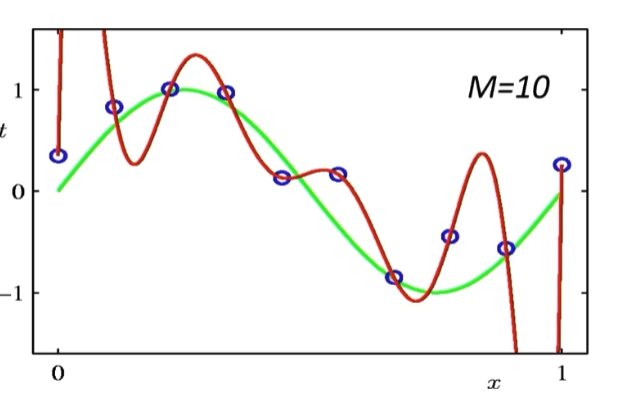
\includegraphics{/Users/fanqiulin/Desktop/cse-545_ML-notes/lec-notes/Linear_Regression.assets/Screenshot 2025-01-21 at 18.11.37.png}

overfitting 的原因: features 数量 M 设置得太多, 导致过度保持 training
sets 的点靠近曲线, 但是对于 testing set 并不对( 这里是一个简化,
实则不能单纯这样划分, 需要 cross validation)

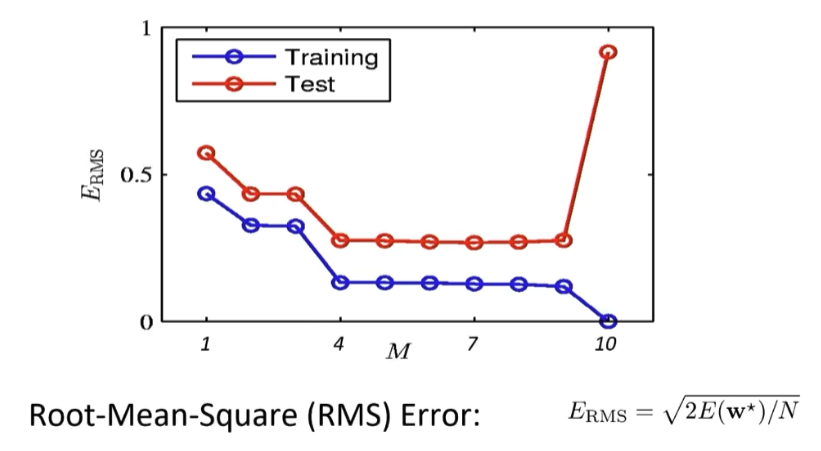
\includegraphics{/Users/fanqiulin/Desktop/cse-545_ML-notes/lec-notes/Linear_Regression.assets/Screenshot 2025-01-21 at 18.11.50.png}

overfitting 的表现: 各项 features 的参数动荡很大.

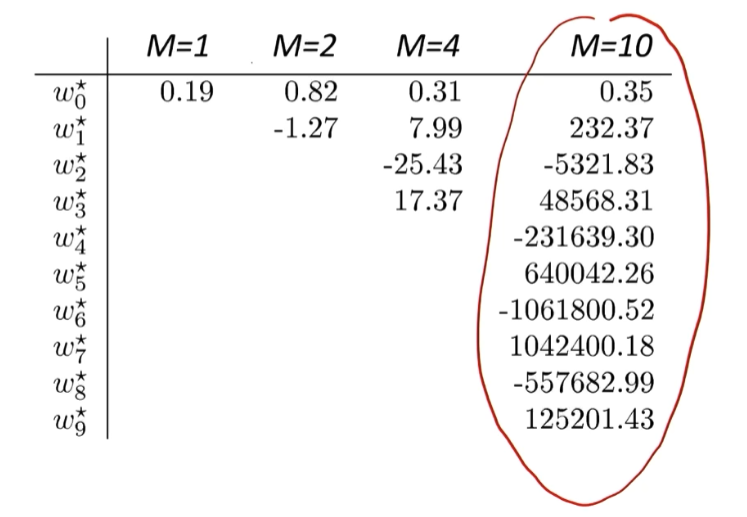
\includegraphics{/Users/fanqiulin/Desktop/cse-545_ML-notes/lec-notes/Linear_Regression.assets/Screenshot 2025-01-21 at 18.12.41.png}

overfitting 的解决方法 1: 增加数据点

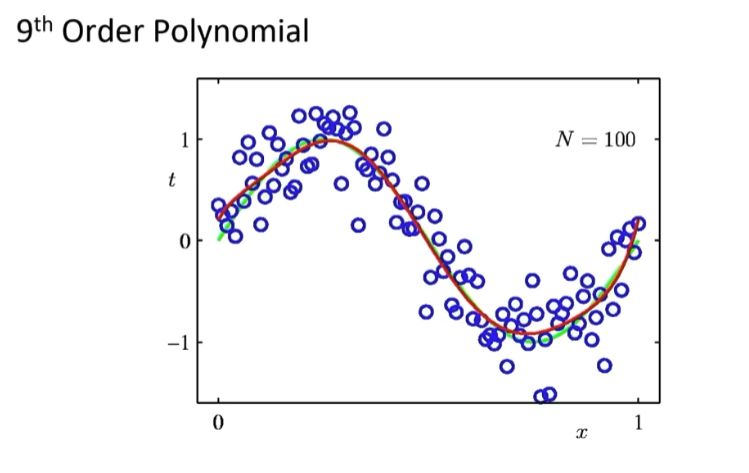
\includegraphics{/Users/fanqiulin/Desktop/cse-545_ML-notes/lec-notes/Linear_Regression.assets/Screenshot 2025-01-21 at 18.13.03.png}

overfitting 的解决方法 2:

\hypertarget{regularization-solving-overfit}{%
\paragraph{regularization: solving
overfit}\label{regularization-solving-overfit}}

我们通过引入一个 regularization term, 也称为 penalty term 惩罚项,
以使得曲线尽量平缓, 从而减少 overfitting.

Idea: 把 \(w\) 本身的 Magnitute 作为一个 loss function 的一部分,
让我们降低 loss 的同时自带降低 w 的各个 entries 的正负动荡程度,
从而使得拟合曲线尽量平缓, 降低曲线的 expressibility.

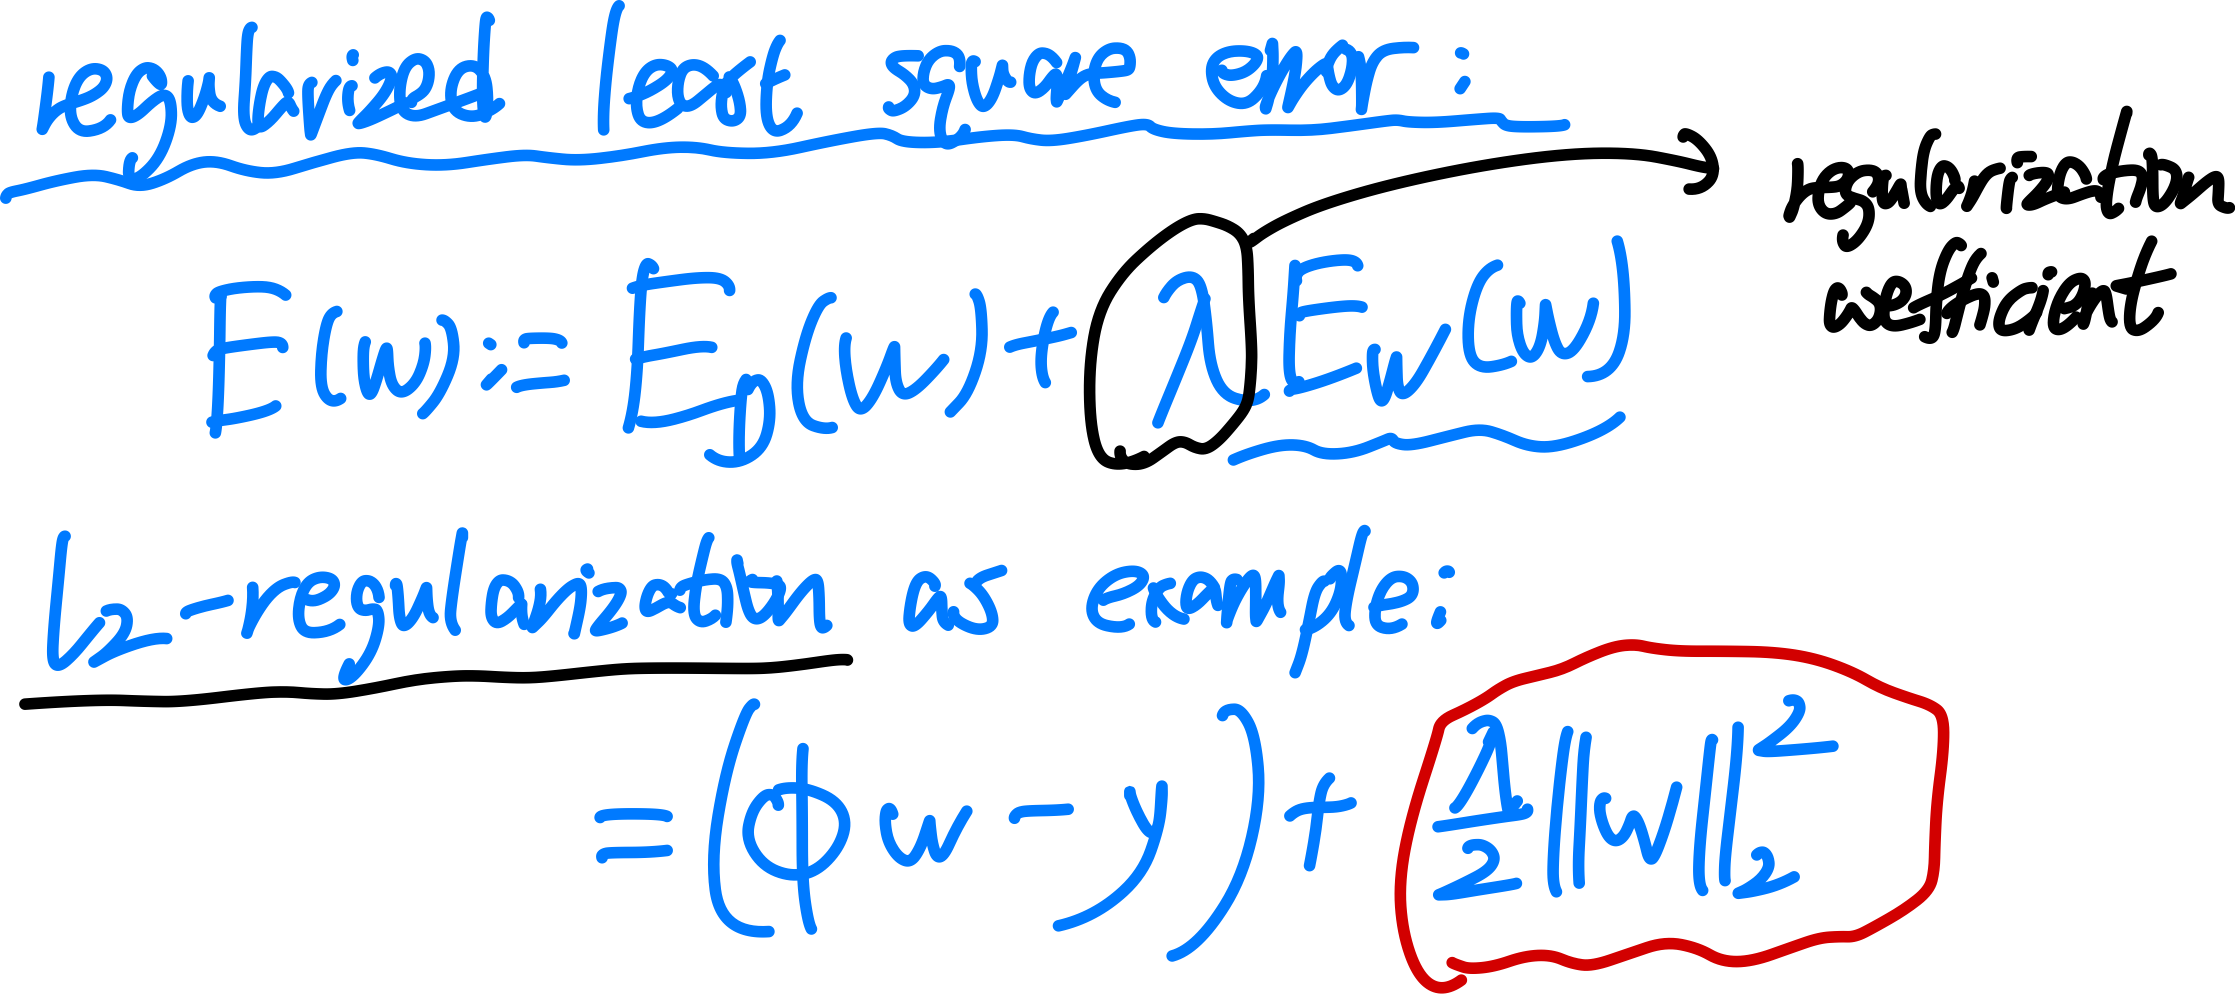
\includegraphics{/Users/fanqiulin/Desktop/cse-545_ML-notes/lec-notes/Linear_Regression.assets/image-20250121201523836.png}

这里的 \(\lambda\) 理应设置较小, 如 0.001 等.

\(\lambda\) 设置越大, 曲线越接近 constant. 比如 \(\lambda := 1\), 则会

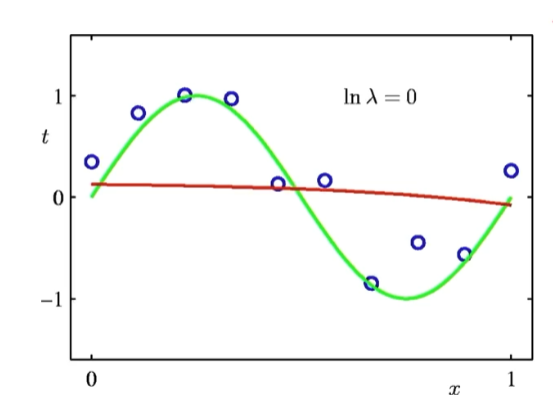
\includegraphics{/Users/fanqiulin/Desktop/cse-545_ML-notes/lec-notes/Linear_Regression.assets/Screenshot 2025-01-21 at 20.17.21.png}

如果 traning error 和 testing error 都很大, 那就说明 \(\lambda\)
调太大了.

\hypertarget{gradient-of-regularized-least-square}{%
\paragraph{gradient of regularized least
square}\label{gradient-of-regularized-least-square}}

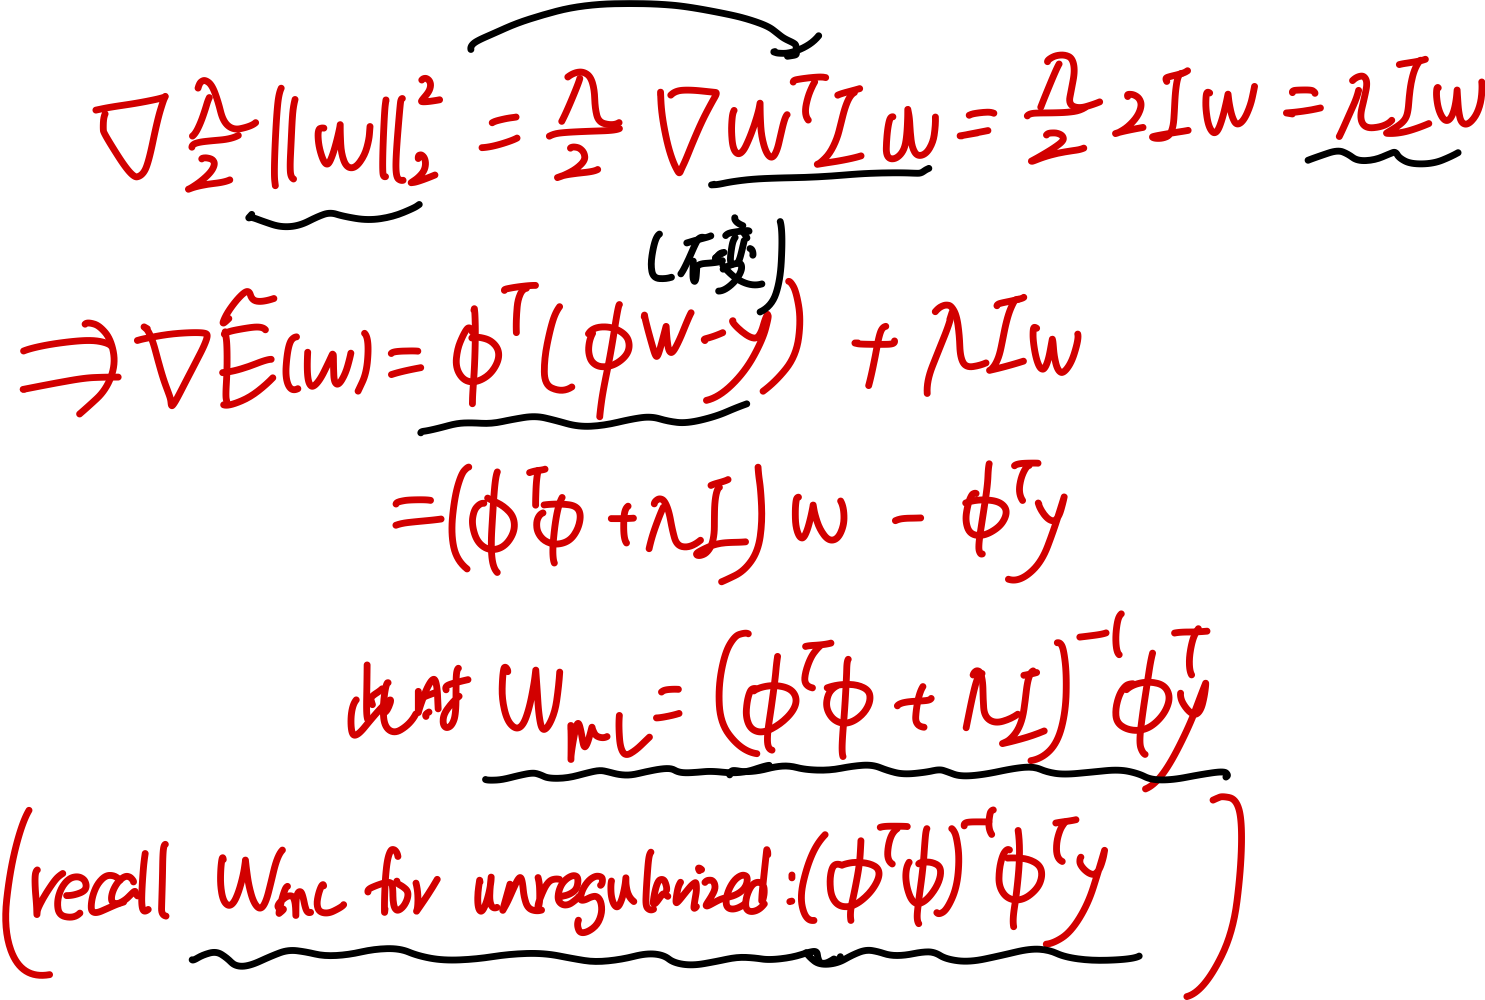
\includegraphics{/Users/fanqiulin/Desktop/cse-545_ML-notes/lec-notes/Linear_Regression.assets/image-20250121204803377.png}

summary: regularization controls the tradeoff bewteen fitting error 和
expressibility.

\hypertarget{linear-regressionlec3}{%
\subsection{Linear Regression(lec3)}\label{linear-regressionlec3}}

\hypertarget{review-on-probability}{%
\subsubsection{Review on Probability}\label{review-on-probability}}

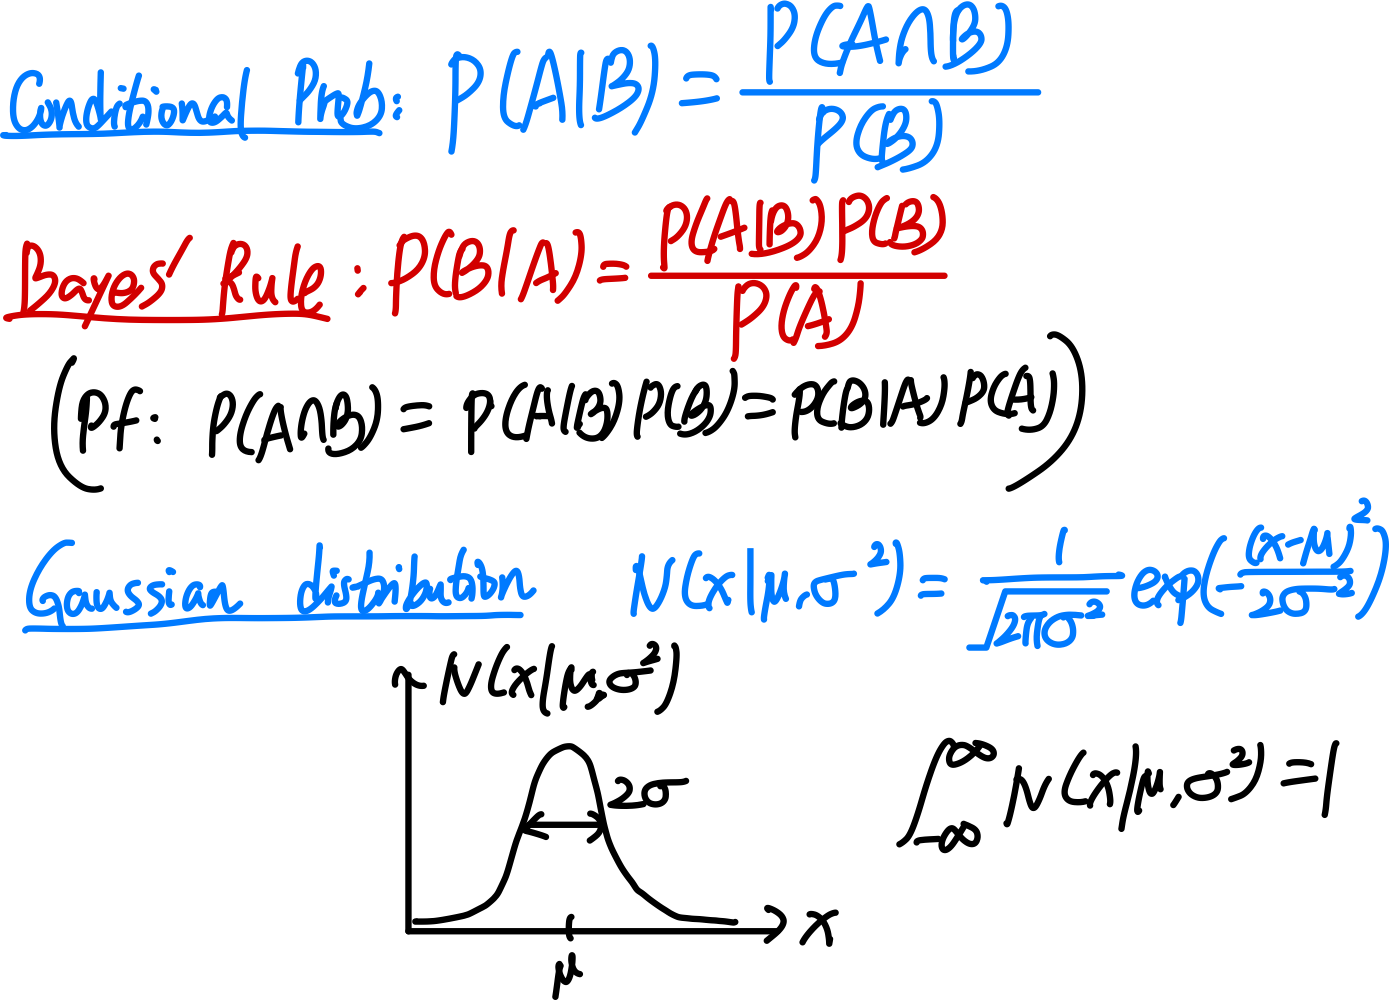
\includegraphics{/Users/fanqiulin/Desktop/cse-545_ML-notes/lec-notes/Linear_Regression.assets/image-20250121215444693.png}

\hypertarget{likelihood-function}{%
\paragraph{Likelihood function}\label{likelihood-function}}

\textbf{Likelihood function} (似然函数) 表示在给定一组 i.i.d 的数据
samples \(D\) 以及其以 \(\theta\) 为参数的分布形式下,random vector
=\(D\) 处的概率密度;其以参数 \(\theta\) 为变量,表达的是在固定数据
\(D\) 的前提下,不同参数 \(\theta\) 对数据的适配程度

而 maximum likelihood estimator 则是使得这个 random vector =\(D\)
处的概率密度 maximize 的参数 \(\tilde{\theta}\)

由于独立同分布, random vector =\(D:=\{x_1,\cdots,x_n\}\)
处的概率密度就等于所有 \(X=x_i\) 处的概率密度的 product.

取得 maximum likelihood estimator 即: 在这个参数下, 我们得到的模型,
对于我们的训练数据而言, 取得其相对的 y 的概率密度最大.

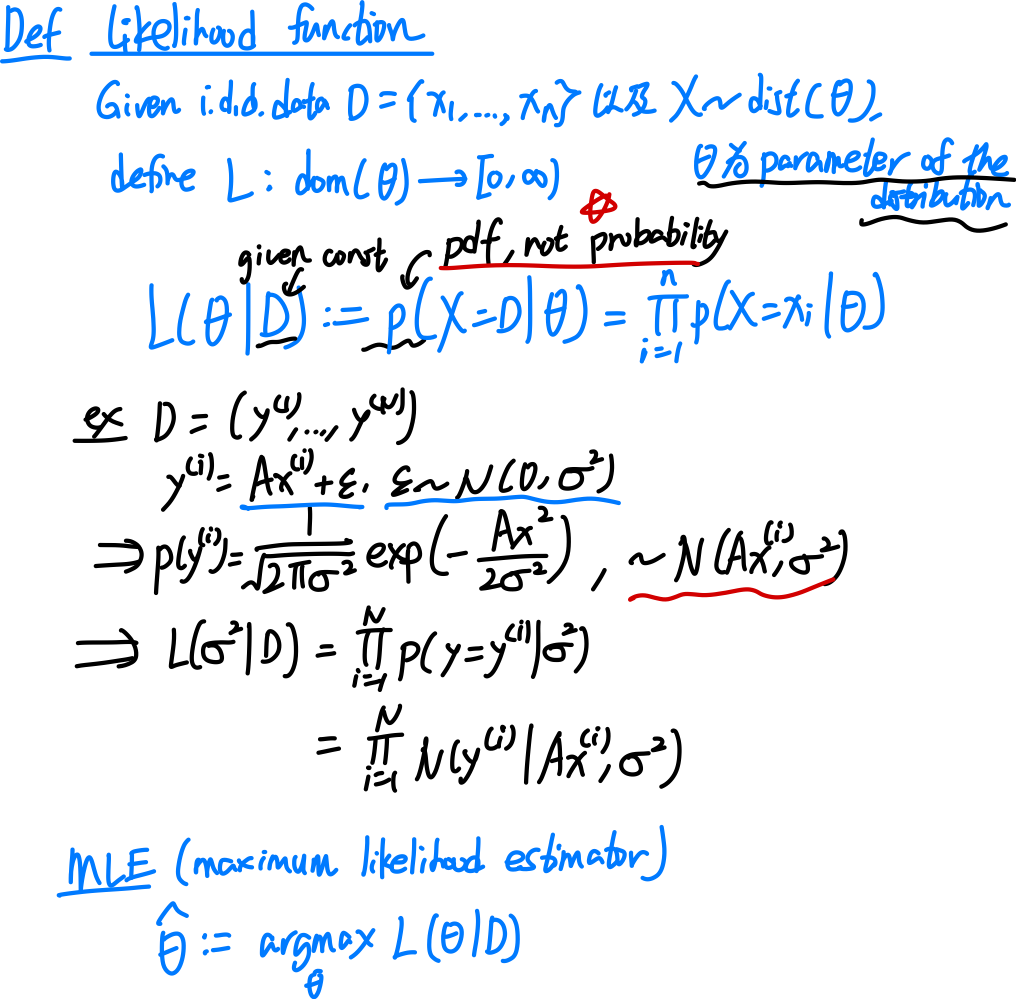
\includegraphics{/Users/fanqiulin/Desktop/cse-545_ML-notes/lec-notes/Linear_Regression.assets/image-20250123174328307.png}

\hypertarget{find-mle-for-linear-model-with-stochastic-noise}{%
\subsubsection{Find MLE for linear model with stochastic
noise}\label{find-mle-for-linear-model-with-stochastic-noise}}

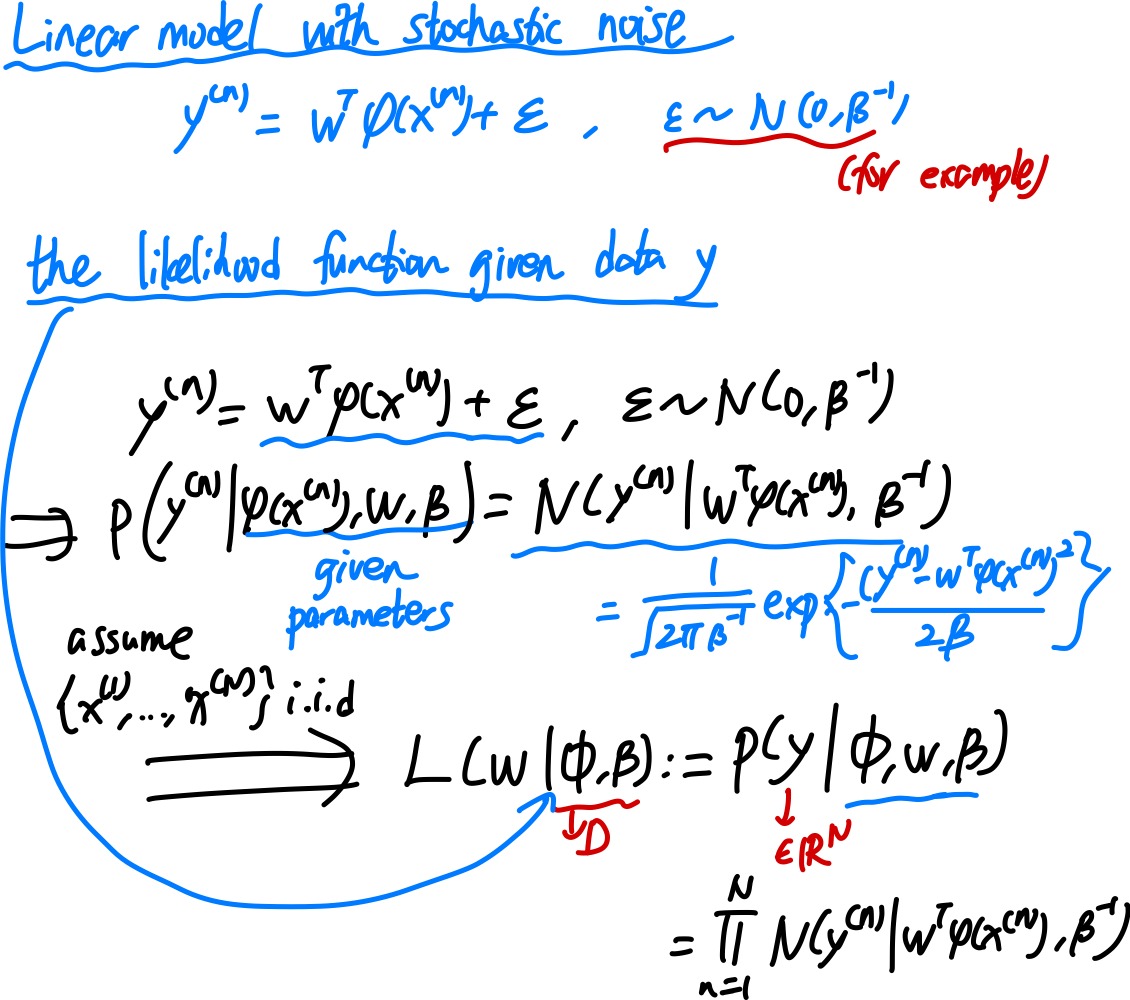
\includegraphics{/Users/fanqiulin/Desktop/cse-545_ML-notes/lec-notes/Linear_Regression.assets/image-20250123180811150.png}

(求解MLE 可得: linear model with stochastic noise which is normal
distributed centered at 0 得到的 MLE,与标准的 linear model 得到的 MLS
最优解是等价的.

这是符合直觉的,因为一个正态分布的 noise 不影响参数的选择)

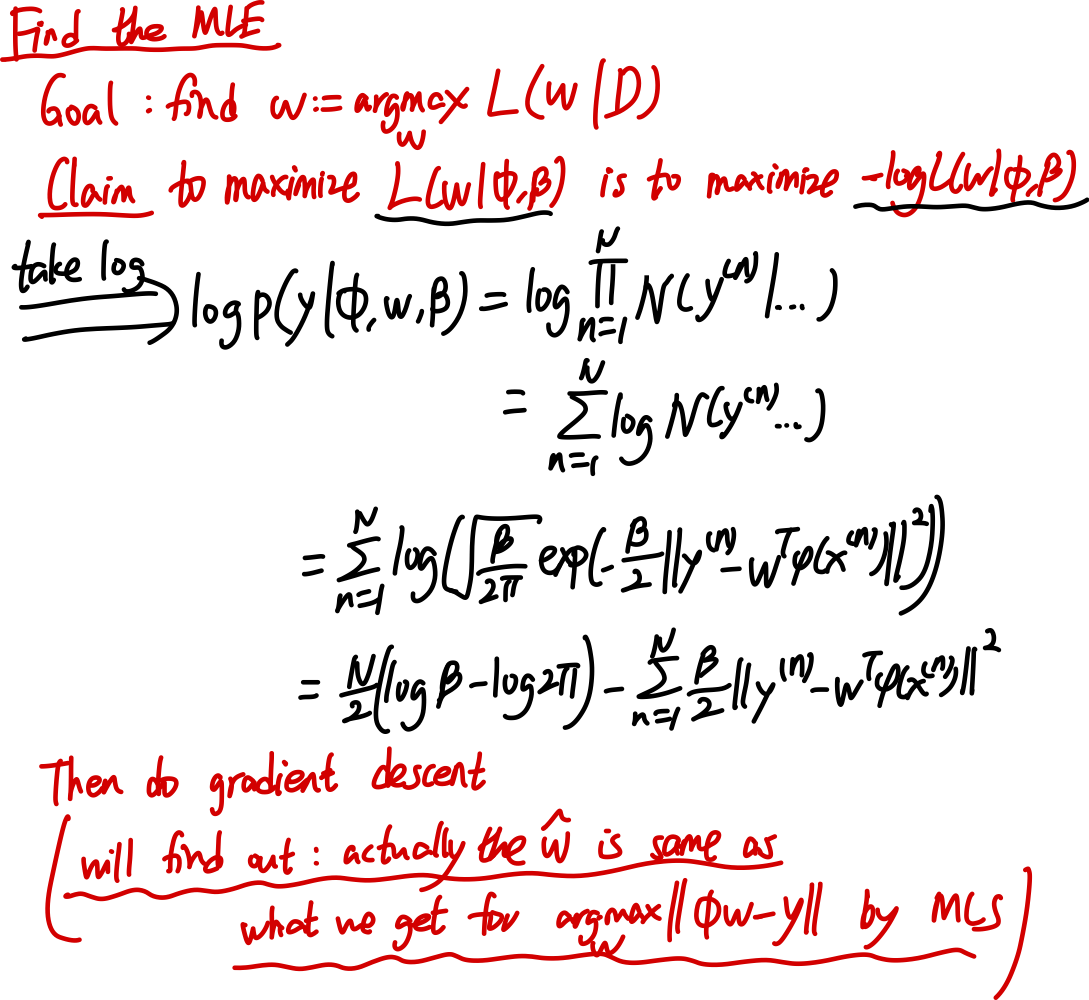
\includegraphics{/Users/fanqiulin/Desktop/cse-545_ML-notes/lec-notes/Linear_Regression.assets/image-20250123180955714.png}

\hypertarget{locally-weighted-linear-regression}{%
\subsubsection{\texorpdfstring{locally weighted linear regression
}{locally weighted linear regression }}\label{locally-weighted-linear-regression}}

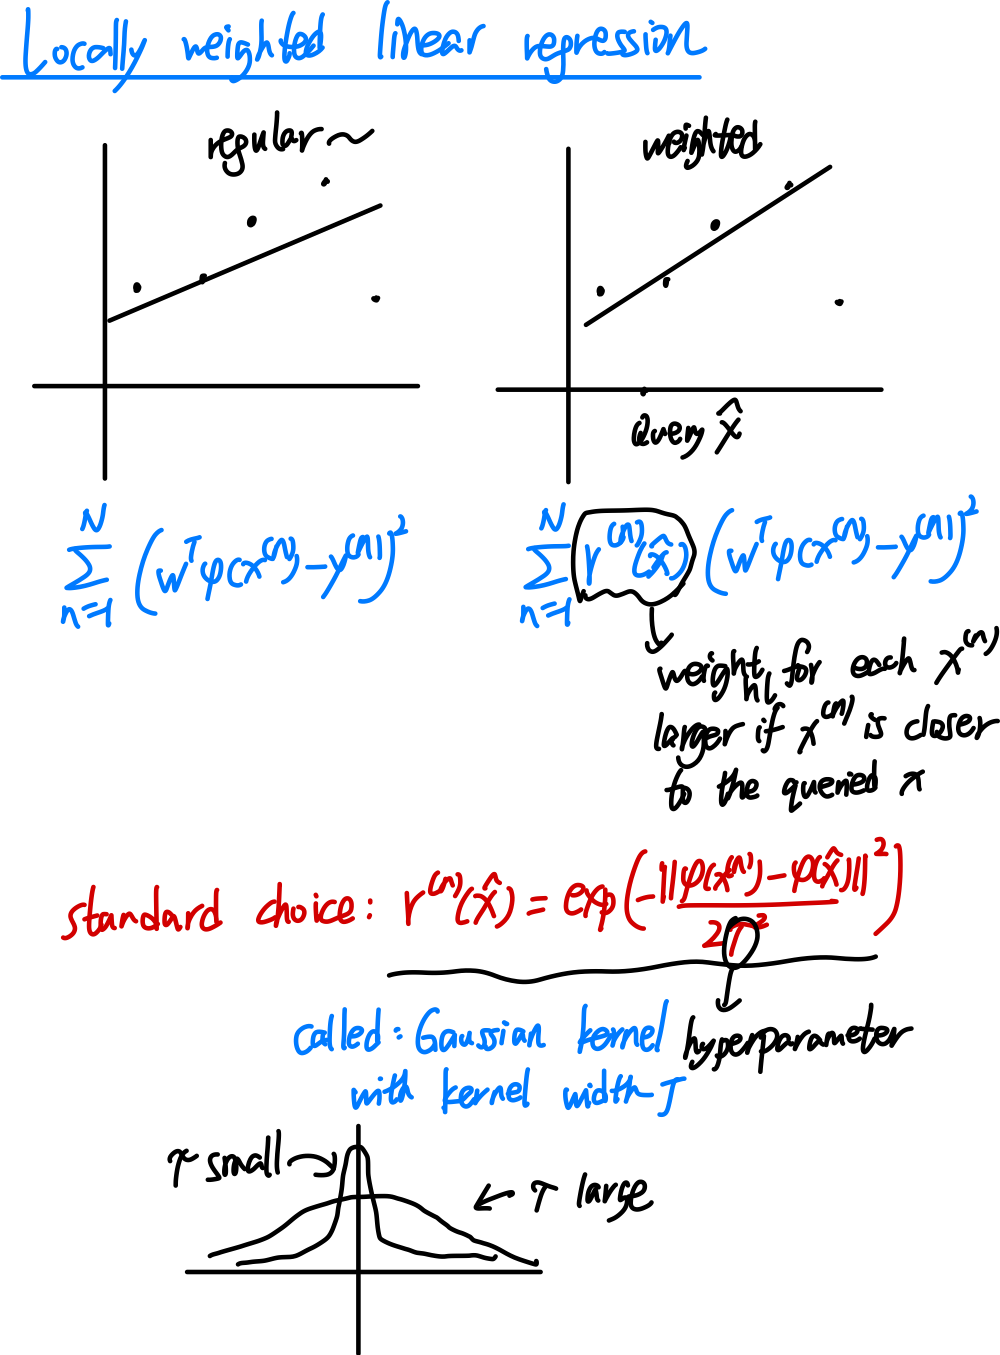
\includegraphics{/Users/fanqiulin/Desktop/cse-545_ML-notes/lec-notes/Linear_Regression.assets/image-20250123193833909.png}

\end{document}
